In diesem Kapitel wird beschrieben wie das semantische Schema einer typische OLTP-Anwendung, also ein System welches traditionell mit relationalen Datenbanken arbeitet, in ein Graph-Schema von MariaDBs OQGRAPH überführt werden kann. Als Beispiel dient ein Diskussionsforum, in dem Mitglieder Beiträge verfassen und kommentieren können. Abbildung \ref{fig:semanticSchema} zeigt das semantische Schema des Forums. In den folgenden Abschnitten wird das ensprechnde Datenbankschema konzipiert, sowie diverse typische Usecases für ein solches Forum erläutert und implementiert. Die Verwendung dieser Usecases erfolgt über einem entferntem PHP-Client, welcher ebenfalls kurz vorgestellt wird.

\begin{figure}
	\centering
	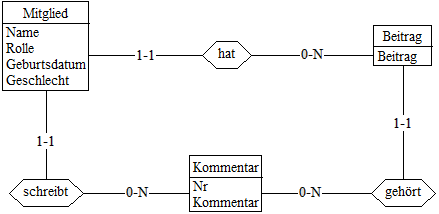
\includegraphics[width=0.6\textwidth]{images/semantischesSchema.png}	
	\caption{Semantisches Schema der Beispielwendung: Diskussionsforum}
	\label{fig:semanticSchema}
\end{figure}

\subsection{Konzeption des Schema}
OQGRAPH wird als Engine beschrieben, welche dem Nutzer die Handhabung hierarchische Strukturen (Bäume) und komplexe Graphen (zahlreiche Kanten) ermöglichen soll \cite{oqgraph}. Dieser Aussage wird OQGRAPH, insbesondere im erstem Punkt, nicht gerecht. Die Grundlegende Funktionsweise des Systems wird in Kapitel \ref{chp:funktionsweise} beschrieben.

Das Kernproblem von OQGRAPH, welches die Modellierung hierarchischer Strukturen betrifft, ist das Knoten nicht, beziehungsweise nicht explizit gespeichert werden. Lediglich ein numerischer Wert welcher den Knoten repräsentiert wird vorgehalten. Die resultiert in zwei Problemen. Zum einen kann nicht zwischen unterschiedlichen Knotenausprägungen (z. B. Kommentar und Beitrag) unterschieden werden. Dementsprechend ist es auch nicht möglich Knoten bei der Traversierung zu filtern. 

Zum anderen werden die Knoten in OQGRAPH durch eine globale Objektinstanz repräsentiert. Relationale Schema arbeiten aber typischerweise mit einen lokalen Identifikator. Das heißt es ist ein explizites Mapping nötig, wenn der OQGRAPH Knoten mit dem zugehörigen Nutzdatensatz in Verbindung gebracht werden soll. Möchte man diese Daten also zusammenführen ist ein Join notwendig. Graphdatenbanken sind aber so performant weil es eben nicht nötig ist Datensätze zu über einen Join zusammenzuführen.

Aufgrund dieser Limitierungen ist OQGRAPG ungeeignet für die Umsetzung komplexer Schemata. Um dies weiter auszuführen wurde ein OQGRAPH kompatibles Schema erstellt. In wie fern damit Usecases umgesetzt werden können, beziehungsweise wie Workarounds aussehen und mit Limitierungen umzugehen ist, wird in den folgenden Abschnitten vorgestellt.

Abbildung \ref{fig:logicSchema} zeigt das konzeptionelle Schema unserer Beispielanwendung Diskussionsforum. Die drei Objekte Mitglied, Benutzer und Kommentar werden in relationalen Tabellen gespeichert und bekommen einen lokal gültigen Primärschlüssel. Aber anstatt eines Fremdschlüssels auf die entsprechende Beziehungstabelle halten diese eine global eindeutige Objektidentität vor welche in der Backing-Tabelle von OQGRAPH verwendet werden. Dieser Identifier wird durch eine separate Sequenz verwaltet, ein Index auf diesem ermöglicht des Weiteren schnelles Auffinden der Nutzdaten zu den von dem Graphalgohritmus gefundenen Ergebnissen. Die Relationen werden also als Kanten durch das OQGRAPH verwaltet, zu den eigentlichen Kanten (Start/Endknoten, Gewicht) wird auch Relationstyp gespeichert, so das bekannt ist welcher Ausprägung der Zielknoten hat und so die Nutzdaten direkt aus der entsprechenden Tabelle geladen werden können. Da die referenzierte Nutzdatentabelle über den Relationstyp aufgelöst werden muss, kann auch nicht durch die DB referentielle 
Integrität gewährleistet werden.

\begin{figure}	
	\centering
	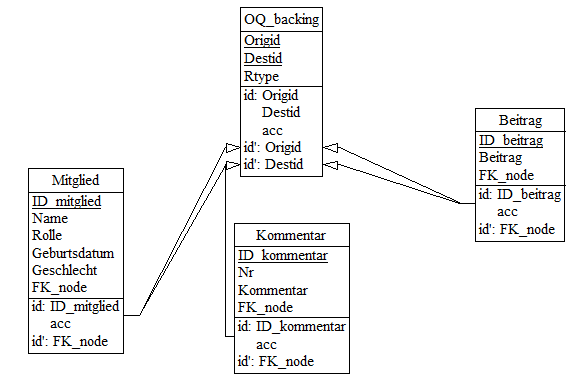
\includegraphics[width=0.9\textwidth]{images/logischesSchema.png}
	\caption{Logisches Schema der Beispielwendung: Diskussionsforum}
	\label{fig:logicSchema}
\end{figure}
 
Das komplette SQL-Schema, sowie des Installationsprotokoll auf dem Hochschulrechner, ist im Anhang \ref{todo} zu finden.

\subsection{Umsetzung eines Clients}
Bei der Entwicklung eines Clients für die Graph-Datenbank des Gästebuchsystems wurde sich für eine Webanwendung entschieden. Webanwendungen können über den Webbrowser aufgerufen und genutzt werden. Sie stehen damit einer Vielzahl von Nutzern zur Verfügung. Ein weiter Vorteil von Webanwendungen ist, dass die Entwicklung des User Interfaces nicht sehr aufwendig ist. Es müssen lediglich gängige Technologien der Webentwicklung für User Interfaces herangezogen werden, die dann schließlich vom Webbrowser interpretiert werden.

Der Client teilt sich auf in die die server-seitige Datenbereitstellung, sowie der client-seitige Datendarstellung.

\subsubsection{Datenbereitstellung}
Die Datenbereitstellung hat die Aufgabe mit der Datenbank zu kommunizieren und die Daten für die Datendarstellung aufzubereiten. Zur Entwicklung der Datenbereitstellung wurde die Skriptsprache PHP gewählt. Bei der Architektur des Systems wurde auf das im Software Engineering gängige Model-View-Control-Pattern (MVC) zurückgegriffen.

Neben den verschiedenen MVC-System-Komponenten ist die Datenbank-Kommunikation eine sehr wichtige Service-Komponente. Bei dem \grqq mysqlConnect\grqq{} handelt es sich um die PHP-Klasse, die die Kommunikation mit der Datenbank abwickelt. Dabei nutzt die mysqlConnect-Klasse die MySQLi-Erweiterung von PHP \cite{PHP-Mysqli}. Eine Erweiterung von PHP im speziellen für MariaDB oder sogar für die Store-Enginge OQGRAPH gibt es nicht. Dafür ermöglicht die MySQLi-Erweiterung das Absetzen von regulären, aber auch von OQGRAPH entsprechende SQL-Befehle \cite{PHP-Mysqli-Query}. Neben der Ausführung diverser SQL-Befehle unterstützt die MySQLi-Erweiterung auch die Interpretation der Antwort der Datenbank. Sogenannte Fetch-Operationen lesen dabei alle Zeilen der Antwort-Tabelle ein und erlauben damit PHP eine Verarbeitung der entsprechenden Zeilen \cite{PHP-Mysqli-Fetch}.

Als Service-Komponente bietet die mysqlConnect-Klasse den Service der Kommunikation mit der Datenbank an. Sie ist in der Datenbereitstellung die einzige Stelle, die eine Kommunikation mit der Datenbank erlaubt. Das bedeutet also auch, dass sich die Nutzer der mysqlConnect-Klasse nicht mehr um die datenbank-spezifische Kommunikation kümmern müssen. Dafür muss die mysqlConnect-Klasse aber auch alle nötigen Zusicherungen erfüllen, da sich die Nutzer unter Angabe von Parametern darauf verlassen müssen, dass sie die gewünschten Daten erhalten. Solange diese Zusicherung erfüllt wird ist es für den Nutzer nicht relevant wie genau die Zusicherung implementiert wird. So kann beispielsweise die Kommunikationsart oder gar die ganze Datenbank ausgetauscht werden, ohne dass Änderungen im übrigen System notwendig werden. Änderungen im Schema der Datenbank betreffen so beispielsweise allein die mysqlConnect-Klasse. Hierbei handelt es sich also um das Adapter-Pattern.

Die mysqlConnect-Klasse beinhaltet alle Operationen bezüglich des CREATE, READ, UPDATE und DELETE (CRUD) in Bezug auf Mitglieder, Beiträge und Kommentare. Darüber hinaus besitzt die mysqlConnect-Klasse speziellere Leseoperationen, bspw. im Bezug auf die Kantenbeziehungen zwischen einzelnen Knoten. Für die Datenbereitstellung wurden jedoch keine Funktionen von OQGRAPH genutzt (siehe \ref{OQGRAPH-Client} \nameref{OQGRAPH-Client}).

\begin{figure}	
	\centering
	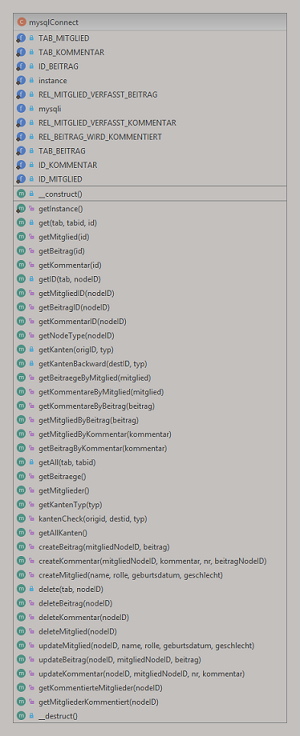
\includegraphics[width=0.6\textwidth]{images/mysqlConnect2.png}
	\caption{UML-Diagramm der Klasse \grqq mysqlConnect\grqq{} (erstellt mit PHPStorm)}
\end{figure}

Die verschiedenen Knoten Mitglieder, Beiträge und Kommentare sind als Model-Klassen implementiert worden. Aus ihnen können Objekte generiert werden, die die jeweiligen Elemente, aber auch die Knoten darstellen. Für die Erstellung des Objektes wird die jeweilige Objekt-ID benötigt. Sollte nur die jeweilige Knoten-ID vorliegen, kann mittels des mysqlConnect-Adapters die zugehörige Objekt-ID ermittelt werden.

Die View-Komponenten liefern die nötigen Informationen an die Datendarstellung. Hierfür nutzen die View-Komponenten den mysqlConnect-Adapter, sowie die verschiedenen Model-Klassen und den darauß resultierenden Objekten. Sie bieten der Darstellungen unter anderem die CRUD-Operationen auf die Graph-Datenbank an, dessen Anfragen und Aufgaben an den mysqlConnect-Adapter weitergereicht werden. Die verschiedenen View-Komponenten resultieren aus den entsprechenden Use Cases, die in \ref{Datendarstellung} \nameref{Datendarstellung} beschrieben werden.

\subsubsection{Datendarstellung}\label{Datendarstellung}

Die Datendarstellung teilt sich in die Sicht der Beiträge und Kommentare, sowie in die Sicht eines einzelnen Mitgliedes auf. Die Sicht der Beiträge und Kommentare listet alle aktuellen Beiträge auf und stellt zu jedem Beitrag seine Kommentare dar. In dieser Sicht ist es ebenso möglich, Beiträge und Kommentare, aber auch Mitglieder zu erstellen. Die Sicht eines einzelnen Mitgliedes stellt die Informationen und Statistiken über das einzelne Mitglied dar. Beide Sichten erfüllen dabei einige der im Projektplan dargelegten Use Cases.

Bei der Entwicklung der Sichten wurden Webkomponenten entwickelt. Bei Webkomponenten handelt es sich um JavaScript-Objekte, die vom Webbrowser interpretiert werden und deswegen dynamisch geladen, erzeugt und aktualisiert werden können. Dabei nutzen die Webkomponenten beim Laden der Webseite die View-Komponenten der Datenbereitstellung, um darzustellende Informationen zu erhalten, zu speichern und anzuzeigen.

Eine Webkomponente stellt dabei unter anderem einen einzigen Beitrag oder einen Kommentar dar. Diese Webkomponenten werden durch speziell definierte HTML-Tags und der jeweiligen Objekt-ID generiert. Es gibt aber auch Webkomponenten für das Erstellen, Bearbeiten, Ansehen und Löschen von Mitgliedern, Beiträgen und Kommentaren.

Folgende Use Cases wurden umgesetzt:
\begin{itemize}
	\item \textbf{Einfügen neuer Mitglieder, Beiträge und Kommentare}: Hierfür werden die Webkomponenten \grqq gb-neu-beitrag.js\grqq{}, \grqq gb-neu-kommentar.js\grqq{} und \grqq gb-neu-mitglied.js\grqq{} genutzt. Für das Erstellen der jeweiligen Elemente werden die View-Komponenten \grqq createBeitrag.php\grqq{}, \grqq createKommentar.php\grqq{} und \grqq createMitglied.php\grqq{} genutzt. Für das Erstellen von Beiträgen und Kommentaren ist das entsprechende Mitglied notwendig. Die Webkomponenten für das Erstellen von Beiträgen und Kommentaren erhalten die entsprechenden Mitglieder von den View-Komponenten \grqq getMitglied.php\grqq{} und \grqq getMitglieder.php\grqq{}. Die Webkomponenten werden in der Sicht für Beiträge und Kommentare genutzt. Das Erstellen von Kommentaren ist aber auch in der Sicht über einzelne Mitglieder möglich.
	\item \textbf{Löschen von Mitglieder, Beiträge und Kommentare}: Die Webkomponenten \grqq gb-beitrag.js\grqq{} und \grqq gb-kommentar.js\grqq{} beinhalten einen Button, mittels dem der zugehörige Beitrag oder Kommentar gelöscht werden kann. Das Löschen von Beiträgen und Kommentaren ist sowohl in der Sicht für Beiträge und Kommentare, als auch in der Sicht über einzelne Mitglieder möglich. Für das Löschen von Mitgliedern gibt es eine eigene Webkomponente \grqq gb-loeschen-mitglied.js\grqq{} in der Sicht von Beiträgen und Kommentaren. Für das Löschen werden die View-Komponenten \grqq deleteBeitrag.php\grqq{}, \grqq deleteKommentar.php\grqq{} und \grqq deleteMitglied.php\grqq{} entsprechend genutzt.
	\item \textbf{Ändern von Mitgliedern, Kommentaren und Beiträgen}: Hierfür werden in den Webkomponenten \grqq gb-beitrag.js\grqq{} und \grqq gb-kommentar.js\grqq{} Buttons zur Bearbeitung angeboten. Außerdem bietet die Webkomponente \grqq gb-loeschen-mitglied.js\grqq{} nicht nur eine Option für das Löschen, sondern auch für das Bearbeiten von Mitgliedern an. Die tatsächliche Bearbeitung findet dann in den Komponenten \grqq gb-neu-beitrag.js\grqq{}, \grqq gb-neu-kommentar.js\grqq{} und \grqq gb-neu-mitglied.js\grqq{} statt, die dann zur Bearbeitung umfunktioniert werden. Zur Speicherung der Änderung werden die View-Komponenten \grqq updateBeitrag.php\grqq{}, \grqq updateKommentar.php\grqq{} und \grqq updateMitglied.php\grqq{} genutzt.
	\item \textbf{Anzeige und Anzahl der Kommentare ausgewählter Beiträge}: Die Webkomponente \grqq gb-beitrag.js\grqq{} stellt einen einzelnen Beitrag dar. Dazu führt es auch die zugeordneten Kommentare mit der Webkomponente \grqq gb-kommentar.js\grqq{} auf. Es nutzt dafür unter anderem die View-Komponenten \grqq getBeitrag.php\grqq{}, \grqq getKommentar.php\grqq{}, sowie \grqq getMitglied.php\grqq{}.
	\item \textbf{Anzeige und Anzahl der Beiträge ausgewählter Mitglieder}: In der Sicht über einzelne Mitglieder werden dessen Beiträge aufgelistet, sowie deren Anzahl aufgeführt. Hierfür wird die Webkomponente \grqq gb-mitglied-beitraege.js\grqq{} genutzt, die wiederum die View-Komponenten \grqq getBeitraegeByMitglied.php\grqq{} nutzt. Für das Anzeigen der Beiträge wird die Webkomponente \grqq gb-beitrag.js\grqq{} genutzt.
	\item \textbf{Anzeige und Anzahl der Kommentare ausgewählter Mitglieder}: Ebenfalls in der Sicht über einzelne Mitglieder werden die Beiträge aufgelistet, die vom jeweiligen Mitglied kommentiert wurden. Hierbei wird auch in der Anzahl der Beiträge und der Anzahl der Kommentare des jeweiligen Mitgliedes differenziert. Hierzu nutzt die Webkomponente \grqq gb-mitglied-kommentar.js\grqq{} die View-Komponente \grqq getKommentareByMitglied.php\grqq{}. Für das Anzeigen der Beiträge wird die Webkomponente \grqq gb-beitrag.js\grqq{} genutzt.
	\item \textbf{Anzeige und Anzahl der kommentierten Beiträge ausgewählter Mitglieder}: Dies wurde bereits im Use Case \grqq Anzeige und Anzahl der Beiträge ausgewählter Mitglieder\grqq{} umgesetzt.
	\item \textbf{Anzeige Anzahl der kommentierten Mitglieder ausgewählter Mitglieder}: Hierfür werden zwei Statistiken angezeigt:
	\begin{enumerate}
		\item Eine Statistik die anzeigt, wie oft das jeweilige Mitglied von einem anderen Mitglied kommentiert wurde. Hierzu wird die Webkomponente \grqq gb-mitglied-von-mitglied.js\grqq{} genutzt, die ihre Informationen von der View-Komponente \grqq getKommentareMitgliedVonMitglied.php\grqq{} erhält. Sie listet zu jedem Mitglied auf, welches Mitglied wie oft das jeweilige Mitglied kommentiert hat.
		\item Eine Statistik darüber, wie oft das jeweilige Mitglied andere Mitglieder kommentiert hat. Die Webkomponente \grqq gb-mitglied-mitglied.js\grqq{} zeigt die Informationen der View-Komponente \grqq getKommentareMitgliedZuMitglied.php\grqq{} an. Dabei gibt die Statistik zu jedem Mitglied die Anzahl der Kommentare an, die das jeweilige Mitglied bei Beiträgen des angegebenen Mitglieds hinterlassen hat.
	\end{enumerate}
\end{itemize}

\subsubsection{OQGRAPH im Bezug auf den Client}\label{OQGRAPH-Client}

Die Funktionalitäten von OQGRAPH wurden bei der Entwicklung des Clients nicht genutzt. Die Gründe dafür sind vielseitig. Zum einen war die Nutzung von OQGRAPH in diesem Anwendungsfall nicht sinnvoll, weil OQGRAPH keine Möglichkeit bietet zwischen einzelnen Knoten-Arten und Kanten-Beziehungen zu unterscheiden. Eine Selektion von Beitragsknoten ist über Funktionalitäten von OQGRAPH nicht möglich - hierfür muss ein reguläres SQL herangezogen werden. Rückschlüsse auf Knoten-Arten sind zwar in der Theorie über die Gewichte der Wege möglich, jedoch nicht immer sinnvoll und aussagekräftig.

Zum anderen ist auch OQGRAPH in einer relationalen Datenbank \grqq gefangen\grqq{}. So gibt es die erreichbaren Knoten, jedoch nicht den Weg an. Beispielsweise wäre bei der Statistik \grqq Mitglied wurde von anderes Mitglied so oft kommentiert\grqq{} der Pfad essentiell, da nur so ermittelt werden kann wie oft ein Mitglied das andere kommentiert hat. Durch die SQL-Erweiterung von OQGRAPH ist es so nur möglich festzustellen, dass ein Mitglied ein anderes kommentiert hat - jedoch nicht, wie oft.

Ein Beispiel aus den Testdaten verdeutlicht das Problem. Das Mitglied \grqq Oliver Higgins\grqq{} hat drei Beiträge verfasst, die insgesamt elf mal kommentiert wurden. Zwei Kommentare davon kommen vom Mitglied \grqq Leon Clemens\grqq{}. Dabei kommentierte Leon Clemens zwei Beiträge jeweils einmal.

\begin{figure}	
	\centering
	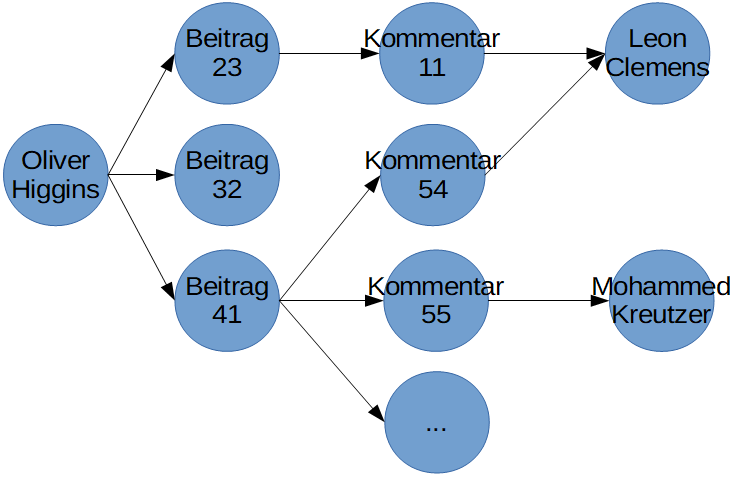
\includegraphics[width=0.6\textwidth]{images/graph.png}
	\caption{Graph zur Kommentiert-Von-Beziehung zwischen Oliver Higgins und Leon Clemens}
\end{figure}

Für die Statistik \grqq Mitglied wurde von anderes Mitglied so oft kommentiert\grqq{} ist es wichtig die Anzahl der Wege zwischen Oliver Higgins und Leon Clemens zu zählen. Diese Funktionalität unterstützt OQGRAPH nicht \cite{OQGRAPH-Examples}. Es ist nur möglich zu ermitteln, welcher Pfad der kürzeste ist oder welche Knoten von welchem Knoten aus erreichbar sind.

\begin{figure}	
	\centering
	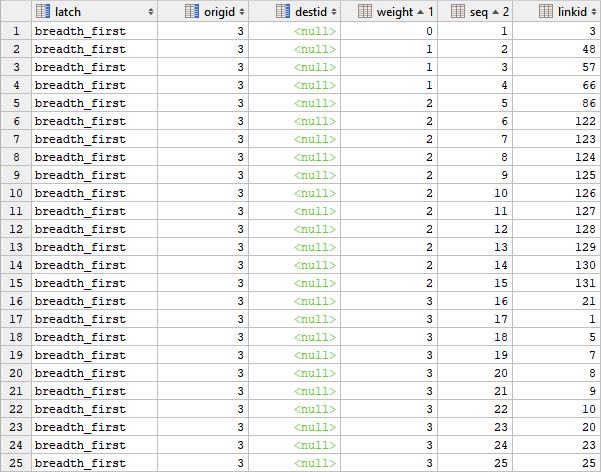
\includegraphics[width=0.7\textwidth]{images/oqgraph-select.png}
	\caption{SQL-Select, wobei origid = 3 hier Oliver Higgins: \newline
		\texttt{SELECT * FROM oq\_graph WHERE latch = 'breadth\_first'\newline AND origid = 3 AND weight < 4}
	}
\end{figure}

Das Ergebnis der Breitensuche stellt uns die im Rahmen der Breitensuche erreichten Knoten dar. Anhand des Vorwissens, dass die origid ein Mitglied ist und in unserem Anwendungsbeispiel es nur Beziehungen der Art Mitglied-Zu-Beitrag, Beitrag-Zu-Kommentar und Kommentar-Zu-Beitrag gibt, können wir darauf schließen, dass die erreichten Knoten mit dem Gewicht (weight) Mitgliedsknoten sein müssen. Wenn jetzt noch eine weitere Beziehung, beispielsweise \grqq Kommentar-Zu-Kommentar\grqq{} hinzukommt, ist ein solcher Schluss nicht mehr möglich. In diesem Fall müsste nach den gefundenen Knoten-IDs nach Treffern in den jeweiligen Knoten-Tabellen gesucht werden.

Das Ergebnis der Anfrage gibt außerdem auch andere Knoten anderer Gewichtungen an. Auch hier lässt sich aus der Gewichtung theoretisch schließen, dass es sich bei den Knoten der Gewichtung 1 um Beitragsknoten und bei Knoten der Gewichtung 2 um Kommentarknoten handelt. Es geht jedoch nicht hervor, in welcher Beziehung die Knoten zueinander stehen. So lässt sich ein Kommentar nicht eindeutig einem Mitglied zuordnen. Hier wäre also eine Tiefensuche sinnvoll, die OQGRAPH zur Zeit jedoch nicht unterstützt.

Auf Grund von fehlenden, für eine Graph-Datenbank jedoch essentielle, Funktionalitäten musste also auf reguläre SQL-Befehle zurückgegriffen werden. Besonderheiten in der Speicherung ergaben sich durch die Formulierung aller Elemente als Knoten, sowie die Speicherung der Beziehungen zwischen den Elementen als Kanten in einer gesonderten, relationalen Tabellen. Auf diese Weise werden jedoch Normalformen verletzt, wodurch es zu Anomalien kommen kann.

\subsection{Fazit}

OQGRAPH kam bei der Realisierung des Gästebuch-Clients nicht zum Einsatz. Grund hierfür ist, dass OQGRAPH eine Erweiterung eines relationalen Datenbanksystems ist. Für viele Abfragen eigneten sich einfache SQL-Abfragen ohne Bezug zu OQGRAPH besser. Da es in OQGRAPH von Grund auf nicht möglich ist Knoten anhand ihres Typs in unterschiedlichen Rekursionsstufen zu filtern und anschließend zu traversieren, wäre eine Umsetzung der Abfragen in OQGRAPH äußerst komplex und definitiv nicht praktikabel gewesen. Die Erweiterung OQGRAPH eignet sich deshalb nur für die Anwendungsfälle, in denen eine Betrachtung von speziellen Knoten- und Kanten-Typen nicht erforderlich ist.